% Standalone rendering of every data figure and table in the AI-Native
% Academia workshop paper (Measurable Writing Standards for AI-Native Venues),
% so the figure and table sources in this repository can be built and checked
% without the manuscript, which is not distributed.
%
%   python paper/ai_native_academia/build_figures.py            # full render, data/ai_native_academia/figures.pdf
%   python paper/ai_native_academia/build_figures.py --public   # the tracked figures.pdf
%
% Build through build_figures.py only: it writes the full render under the
% repository's untracked data/ directory and switches the citation content off
% for the tracked copy.
%
% Data comes from ../../data: pgfplots/ for the figure series shared across
% papers, and ai_native_academia/ for the macros and the generated tables
% (make_macros.py and make_tables.py). The judge heatmap is
% the PNG in ../../shared/figs/, which the UncertaiNLP paper also includes.
% A generated table that was not built, and the citation figure without its
% input, are replaced by a note saying why (the citation outputs need the
% reader's own citation counts). Every other figure needs its input. Captions
% keep their \ref commands, which print as ?? here. The tikz and pgfplots setup matches the manuscript
% preamble, so the figures render as they do there.
\documentclass[10pt]{article}
\usepackage[letterpaper,margin=1in]{geometry}
\usepackage[utf8]{inputenc}
\usepackage[T1]{fontenc}
\usepackage{textcomp}
\usepackage{url}
\usepackage{booktabs}
\usepackage{caption}
\captionsetup[table]{skip=8pt}
\usepackage{amsfonts}
\usepackage{amsmath}
\usepackage{nicefrac}
\usepackage{xcolor}
\usepackage{graphicx}
\usepackage[numbers]{natbib}
\usepackage{tikz}
\usetikzlibrary{arrows.meta, positioning, shapes.geometric, fit, backgrounds}
\usepackage{pgfplots}
\usepackage{pgfplotstable}
\pgfplotsset{compat=1.18,
  every axis/.append style={
    /pgf/number format/1000 sep={},
    /pgf/number format/fixed,
  }
}
\usepgfplotslibrary{groupplots}
\DeclareUnicodeCharacter{2191}{\ensuremath{\uparrow}}
\DeclareUnicodeCharacter{2193}{\ensuremath{\downarrow}}

% The manuscript marks revised text with these for its review build; here
% they print their argument unchanged, as in the published paper.
\newcommand{\rev}[1]{#1}
\newcommand{\revtwo}[1]{#1}
\newcommand{\revthree}[1]{#1}
\newcommand{\revfour}[1]{#1}

\newcommand{\aadata}{../../data}
\newcommand{\aanote}[1]{\begin{center}\fbox{\parbox{0.9\linewidth}{\small #1}}\end{center}}
% \aainput{file}{what}{why}: input file, or a note when it was not built.
\newcommand{\aainput}[3]{\IfFileExists{#1}{\input{#1}}{\aanote{#2 not rendered: #3}}}
\newcommand{\aamacros}[1]{\IfFileExists{\aadata/ai_native_academia/#1}{\input{\aadata/ai_native_academia/#1}}{}}
\aamacros{generated_round2.tex}
\newcommand{\aatable}[2]{\aainput{\aadata/ai_native_academia/tables/#1}{Table \texttt{\detokenize{#1}}}{#2}}
\newcommand{\nocit}{the citation outputs were not built (the citation counts are
  not distributed; see README, Citations)}
\newcommand{\nopipe}{its input was not built; see \texttt{data/incomplete.json}
  and \texttt{data/ai\_native\_academia/}}
% build_figures.py defines \aacitationsabsent when the local citation counts
% are absent, so an output left from an earlier run is not rendered.
\newcommand{\aacitations}[2]{\ifdefined\aacitationsabsent\aanote{#2 not rendered:
  \nocit}\else#1\fi}

\title{abstract-audit: AI-Native Academia figure and table sources}
\author{}
\date{}

\begin{document}
\maketitle

\section*{Main text}

% Flesch Reading Ease on NeurIPS, arXiv ML, arXiv non-ML, and PubMed.
% Data: ../../data/pgfplots/readability_flesch_ease.csv
% Higher values = easier reading.

\begin{figure}[h]
\centering
\begin{tikzpicture}
\begin{axis}[
    width=0.88\linewidth, height=5cm,
    xlabel={Year},
    ylabel={Flesch Reading Ease (\textuparrow\ easier)},
    xtick distance=4,
    x tick label style={rotate=45, anchor=east, font=\tiny,
                        /pgf/number format/1000 sep={}},
    ytick align=inside,
    legend columns=4,
    legend style={draw=none, fill=none, font=\scriptsize,
                  cells={anchor=west}, column sep=8pt,
                  at={(0.5,-0.28)}, anchor=north},
    tick label style={font=\tiny},
    label style={font=\small},
    enlarge x limits=0.02,
  ]
  \addplot[color={rgb,255:red,44;green,160;blue,44}, dashdotted, very thick]
    table[x=year, y=neurips, col sep=comma]
    {../../data/pgfplots/readability_flesch_ease.csv};
  \addlegendentry{NeurIPS}
  \addplot[color={rgb,255:red,148;green,103;blue,189}, solid, very thick]
    table[x=year, y=arxiv_ml, col sep=comma]
    {../../data/pgfplots/readability_flesch_ease.csv};
  \addlegendentry{arXiv ML}
  \addplot[color={rgb,255:red,140;green,86;blue,75}, dotted, thick]
    table[x=year, y=arxiv_nonml, col sep=comma]
    {../../data/pgfplots/readability_flesch_ease.csv};
  \addlegendentry{arXiv non-ML}
  \addplot[color={rgb,255:red,214;green,39;blue,40}, dashed, thick]
    table[x=year, y=pubmed, col sep=comma]
    {../../data/pgfplots/readability_flesch_ease.csv};
  \addlegendentry{PubMed}
  % ChatGPT launch marker (late 2022)
  \draw[black, dashed, semithick] (axis cs:2022,-5) -- (axis cs:2022,50);
  \node[font=\tiny, rotate=90, anchor=south west]
    at (axis cs:2022.2,18) {ChatGPT (2022)};
\end{axis}
\end{tikzpicture}
\caption{\textbf{Flesch Reading Ease on NeurIPS, arXiv ML, arXiv
  non-ML, and PubMed, 1987--2025.}
  Higher values indicate easier reading (\textuparrow).
  NeurIPS falls from approximately 24 in 1987 to approximately
  8 in 2025. arXiv ML follows a similar trajectory. The arXiv
  non-ML baseline declines more slowly, indicating that the
  accelerated decline is specific to ML venues. Vertical dashed
  line marks the late 2022 availability of widely-used
  instruction-tuned writing assistants.}
\label{fig:readability-flesch}
\end{figure}

% Total sensational language per 100 abstract words.
% Data: ../../data/pgfplots/sensational_total.csv

\begin{figure}[h]
\centering
\begin{tikzpicture}
\begin{axis}[
    width=0.88\linewidth, height=5cm,
    xlabel={Year},
    ylabel={Total sensational words per 100},
    xtick distance=4,
    x tick label style={rotate=45, anchor=east, font=\tiny,
                        /pgf/number format/1000 sep={}},
    ytick align=inside,
    legend columns=4,
    legend style={draw=none, fill=none, font=\scriptsize,
                  cells={anchor=west}, column sep=8pt,
                  at={(0.5,-0.28)}, anchor=north},
    tick label style={font=\tiny},
    label style={font=\small},
    enlarge x limits=0.02,
    ymin=0,
  ]
  \addplot[color={rgb,255:red,44;green,160;blue,44}, dashdotted, very thick]
    table[x=year, y=neurips, col sep=comma]
    {../../data/pgfplots/sensational_total.csv};
  \addlegendentry{NeurIPS}
  \addplot[color={rgb,255:red,148;green,103;blue,189}, solid, very thick]
    table[x=year, y=arxiv_ml, col sep=comma]
    {../../data/pgfplots/sensational_total.csv};
  \addlegendentry{arXiv ML}
  \addplot[color={rgb,255:red,140;green,86;blue,75}, dotted, thick]
    table[x=year, y=arxiv_nonml, col sep=comma]
    {../../data/pgfplots/sensational_total.csv};
  \addlegendentry{arXiv non-ML}
  \addplot[color={rgb,255:red,214;green,39;blue,40}, dashed, thick]
    table[x=year, y=pubmed, col sep=comma]
    {../../data/pgfplots/sensational_total.csv};
  \addlegendentry{PubMed}
  % ChatGPT launch marker (line only; the text label appears
  % only in fig:readability-flesch, the first chronological figure).
  \draw[black, dashed, semithick] (axis cs:2022,0) -- (axis cs:2022,30);
\end{axis}
\end{tikzpicture}
\caption{\textbf{Total sensational language per 100 abstract words,
  1987--2025.}
  The NeurIPS total rate rises by approximately 80 percent
  between 2015 and 2025 (from 1.10 to 1.98 per 100 words). The
  arXiv non-ML baseline rises far
  more slowly. The divergence between ML and non-ML venues
  accelerates after the late 2022 availability of
  instruction-tuned writing assistants (vertical dashed line).}
\label{fig:sensational-total}
\end{figure}

% Acronym density -- title (left) and abstract (right).
% Data: ../../data/pgfplots/acronyms_title.csv, acronyms_abstract.csv

\begin{figure}[h]
\centering
\pgfplotsset{
  acro style/.style={
    height=5cm, width=0.47\linewidth,
    xlabel={Year}, ylabel={Acronyms per 100 words},
    xtick distance=4, x tick label style={rotate=45, anchor=east, font=\tiny,
                                          /pgf/number format/1000 sep={}},
    ytick align=inside, ymin=0,
    tick label style={font=\tiny}, label style={font=\small},
    enlarge x limits=0.02,
  }
}
% -- title density: legend collected here ----------------------------------
\begin{tikzpicture}
\begin{axis}[acro style,
  title={\small Titles~[\textdownarrow\ better]},
  legend to name=acrolegend,
  legend columns=5,
  legend style={draw=none, fill=none, font=\scriptsize,
                cells={anchor=west}, column sep=6pt},
]
  \addplot[color={rgb,255:red,44;green,160;blue,44}, dashdotted, very thick]
    table[x=year, y=neurips, col sep=comma] {../../data/pgfplots/acronyms_title.csv};
  \addlegendentry{NeurIPS}
  \addplot[color={rgb,255:red,148;green,103;blue,189}, solid, very thick]
    table[x=year, y=arxiv_ml, col sep=comma] {../../data/pgfplots/acronyms_title.csv};
  \addlegendentry{arXiv ML}
  \addplot[color={rgb,255:red,140;green,86;blue,75}, dotted, thick]
    table[x=year, y=arxiv_nonml, col sep=comma] {../../data/pgfplots/acronyms_title.csv};
  \addlegendentry{arXiv non-ML}
  \addplot[color={rgb,255:red,214;green,39;blue,40}, dashed, thick]
    table[x=year, y=pubmed, col sep=comma] {../../data/pgfplots/acronyms_title.csv};
  \addlegendentry{PubMed}
  \addplot[black, dashed, semithick, domain=1987:2025] {2.40};
  \addlegendentry{Barnett 2020 peak (2.40)}
  \draw[black, dashed, semithick] (axis cs:2022,0) -- (axis cs:2022,100);
\end{axis}
\end{tikzpicture}%
\hfill
% -- abstract density ------------------------------------------------------
\begin{tikzpicture}
\begin{axis}[acro style, title={\small Abstracts~[\textdownarrow\ better]}]
  \addplot[color={rgb,255:red,44;green,160;blue,44}, dashdotted, very thick]
    table[x=year, y=neurips, col sep=comma] {../../data/pgfplots/acronyms_abstract.csv};
  \addplot[color={rgb,255:red,148;green,103;blue,189}, solid, very thick]
    table[x=year, y=arxiv_ml, col sep=comma] {../../data/pgfplots/acronyms_abstract.csv};
  \addplot[color={rgb,255:red,140;green,86;blue,75}, dotted, thick]
    table[x=year, y=arxiv_nonml, col sep=comma] {../../data/pgfplots/acronyms_abstract.csv};
  \addplot[color={rgb,255:red,214;green,39;blue,40}, dashed, thick]
    table[x=year, y=pubmed, col sep=comma] {../../data/pgfplots/acronyms_abstract.csv};
  \addplot[black, dashed, semithick, domain=1987:2025] {2.40};
  \draw[black, dashed, semithick] (axis cs:2022,0) -- (axis cs:2022,100);
\end{axis}
\end{tikzpicture}

\vspace{2mm}
\pgfplotslegendfromname{acrolegend}

\caption{\textbf{Acronym density in titles (left) and abstracts
  (right), 1987 to 2025.}
  Lower values indicate fewer acronyms per word (\textdownarrow\
  better). Dashed black horizontal line marks the Barnett and
  Doubleday science-wide peak of 2.40 per 100 words (2019).
  NeurIPS and arXiv ML diverge from the non-ML control around
  2017 on titles and around 2020 on abstracts.}
\label{fig:acronyms}
\end{figure}

\aacitations{\aatable{citation_readability_top_bottom.tex}{\nocit}}{Table
  citation\_readability\_top\_bottom.tex}
% LLM-as-judge: model-averaged z-scores, one curve per prompt.
% Each curve is the mean of all 6 model z-scores for that prompt.
% Z-scores are standardized to each model's own 1987--2022 baseline.
% Data: ../../data/pgfplots/llm_scores_model_avg_{prompt}.csv

\begin{figure}[h]
\centering
\begin{tikzpicture}
\begin{axis}[
    width=0.88\linewidth, height=5cm,
    xlabel={Year},
    ylabel={Model-averaged readability (z-score)},
    xtick distance=4,
    x tick label style={rotate=45, anchor=east, font=\tiny,
                        /pgf/number format/1000 sep={}},
    ytick align=inside,
    ymin=-2, ymax=5,
    legend columns=3,
    legend style={draw=none, fill=none, font=\scriptsize,
                  cells={anchor=west}, column sep=8pt,
                  at={(0.5,-0.28)}, anchor=north},
    tick label style={font=\tiny},
    label style={font=\small},
    enlarge x limits=0.02,
  ]
  \addplot[color={rgb,255:red,44;green,160;blue,44}, solid, very thick]
    table[x=year, y=avg_z, col sep=comma]
    {../../data/pgfplots/llm_scores_model_avg_simple.csv};
  \addlegendentry{Simple}
  \addplot[color={rgb,255:red,148;green,103;blue,189}, dashed, very thick]
    table[x=year, y=avg_z, col sep=comma]
    {../../data/pgfplots/llm_scores_model_avg_ascb.csv};
  \addlegendentry{ASCB}
  \addplot[color={rgb,255:red,214;green,39;blue,40}, dashdotted, very thick]
    table[x=year, y=avg_z, col sep=comma]
    {../../data/pgfplots/llm_scores_model_avg_own_reasoning.csv};
  \addlegendentry{Own reasoning}
  % Baseline reference at z = 0
  \addplot[black, dotted, thin, forget plot, domain=1987:2024] {0};
  % ChatGPT launch marker (line only; the text label appears
  % only in fig:readability-flesch, the first chronological figure).
  \draw[black, dashed, semithick] (axis cs:2022,-2) -- (axis cs:2022,5);
\end{axis}
\end{tikzpicture}
\caption{\textbf{LLM as judge readability on NeurIPS abstracts,
  1987--2024.}
  Each curve is the mean z-score across all six open-weight
  models for one prompt variant, standardized to each model's
  own 1987--2022 baseline (dotted line at zero).
  All three prompts agree: LLM-judged readability is
  approximately flat before 2022 and rises sharply after the
  availability of instruction-tuned writing assistants (vertical
  dashed line), directly contradicting the classical readability
  decline in Figure~\ref{fig:readability-flesch}.}
\label{fig:llm-judge}
\end{figure}

\clearpage

\section*{Appendix}

\aatable{acronym_reuse_freq.tex}{\nopipe}
% Classical readability appendix, split into two 3-column figures
% to fit within the NeurIPS text width.
% Data: ../../data/pgfplots/readability_<metric>.csv

\providecommand{\readpanel}[3]{%
  \nextgroupplot[title={\tiny #1~[#3]},
                 title style={font=\tiny, yshift=-1.5mm}]
  \addplot[color={rgb,255:red,44;green,160;blue,44}, dashdotted, very thick]
    table[x=year, y=neurips, col sep=comma]{../../data/pgfplots/#2.csv};
  \addplot[color={rgb,255:red,148;green,103;blue,189}, solid, thick]
    table[x=year, y=arxiv_ml, col sep=comma]{../../data/pgfplots/#2.csv};
  \addplot[color={rgb,255:red,140;green,86;blue,75}, dotted, thick]
    table[x=year, y=arxiv_nonml, col sep=comma]{../../data/pgfplots/#2.csv};
  \addplot[color={rgb,255:red,214;green,39;blue,40}, dashed, thick]
    table[x=year, y=pubmed, col sep=comma]{../../data/pgfplots/#2.csv};
  \draw[black, dashed, semithick]
    ({axis cs:2022,0} |- {rel axis cs:0,0})
    -- ({axis cs:2022,0} |- {rel axis cs:0,1});
}

% ── Figure A: 8 readability metrics, 3 by 3 layout (1 blank slot) ────────────
\begin{figure}[htbp]
\centering
\resizebox{\linewidth}{!}{\begin{tikzpicture}
\begin{groupplot}[
    group style={
      group size=3 by 3,
      horizontal sep=8mm,
      vertical sep=12mm,
    },
    width=40mm, height=2.4cm,
    scale only axis,
    xlabel={}, ylabel={},
    xtick distance=12,
    x tick label style={rotate=55, anchor=east, font=\tiny,
                        /pgf/number format/1000 sep={}},
    y tick label style={font=\tiny},
    ytick align=inside,
    enlarge x limits=0.02,
    tick label style={font=\tiny},
  ]
  % First panel: legend collected here
  \nextgroupplot[
    title={\tiny Flesch Ease~[\textuparrow]},
    title style={font=\tiny, yshift=-1.5mm},
    legend to name=readlegend,
    legend columns=4,
    legend style={draw=none, fill=none, font=\scriptsize,
                  cells={anchor=west}, column sep=8pt},
  ]
  \addplot[color={rgb,255:red,44;green,160;blue,44}, dashdotted, very thick]
    table[x=year, y=neurips, col sep=comma]{../../data/pgfplots/readability_flesch_ease.csv};
  \addlegendentry{NeurIPS}
  \addplot[color={rgb,255:red,148;green,103;blue,189}, solid, thick]
    table[x=year, y=arxiv_ml, col sep=comma]{../../data/pgfplots/readability_flesch_ease.csv};
  \addlegendentry{arXiv ML}
  \addplot[color={rgb,255:red,140;green,86;blue,75}, dotted, thick]
    table[x=year, y=arxiv_nonml, col sep=comma]{../../data/pgfplots/readability_flesch_ease.csv};
  \addlegendentry{arXiv non-ML}
  \addplot[color={rgb,255:red,214;green,39;blue,40}, dashed, thick]
    table[x=year, y=pubmed, col sep=comma]{../../data/pgfplots/readability_flesch_ease.csv};
  \addlegendentry{PubMed}
  \draw[black, dashed, semithick]
    ({axis cs:2022,0} |- {rel axis cs:0,0})
    -- ({axis cs:2022,0} |- {rel axis cs:0,1});
  % Remaining 7 panels of part A
  \readpanel{Flesch-Kincaid}{readability_flesch_kincaid}{\textdownarrow}
  \readpanel{Gunning Fog}{readability_gunning_fog}{\textdownarrow}
  \readpanel{SMOG}{readability_smog}{\textdownarrow}
  \readpanel{Dale-Chall}{readability_dale_chall}{\textdownarrow}
  \readpanel{Spache}{readability_spache}{\textdownarrow}
  \readpanel{Coleman-Liau}{readability_coleman_liau}{\textdownarrow}
  \readpanel{ARI}{readability_ari}{\textdownarrow}
  % 9th slot blank for layout
  \nextgroupplot[hide axis, scale only axis, width=40mm, height=2.4cm]
\end{groupplot}
\end{tikzpicture}}

\vspace{2mm}
\pgfplotslegendfromname{readlegend}

\caption{\textbf{Classical readability metrics, part A: Flesch
  family and grade-level formulas, 1987--2025.}
  Arrows indicate the direction of easier reading
  (\textuparrow\ = higher is better; \textdownarrow\ = lower is
  better). Every grade-level metric rises on NeurIPS and arXiv
  ML after 2015 and accelerates after 2020; Flesch Reading Ease
  drops correspondingly. Vertical dashed lines mark the
  late-2022 availability of instruction-tuned writing
  assistants. Part B with the remaining seven metrics appears in
  Figure~\ref{fig:app-readability-b}.}
\label{fig:app-readability}
\end{figure}

% ── Figure B: 7 readability metrics, 3 by 3 layout (2 blank slots) ───────────
\begin{figure}[htbp]
\centering
\resizebox{\linewidth}{!}{\begin{tikzpicture}
\begin{groupplot}[
    group style={
      group size=3 by 3,
      horizontal sep=8mm,
      vertical sep=12mm,
    },
    width=40mm, height=2.4cm,
    scale only axis,
    xlabel={}, ylabel={},
    xtick distance=12,
    x tick label style={rotate=55, anchor=east, font=\tiny,
                        /pgf/number format/1000 sep={}},
    y tick label style={font=\tiny},
    ytick align=inside,
    enlarge x limits=0.02,
    tick label style={font=\tiny},
  ]
  \readpanel{Linsear Write}{readability_linsear_write}{\textdownarrow}
  \readpanel{LIX}{readability_lix}{\textdownarrow}
  \readpanel{RIX}{readability_rix}{\textdownarrow}
  \readpanel{FORCAST}{readability_forcast}{\textdownarrow}
  \readpanel{Pwr--Smnr--Kearl}{readability_powers_sumner_kearl}{\textdownarrow}
  \readpanel{Sentence length}{readability_avg_sentence_length}{\textdownarrow}
  \readpanel{Syllables/word}{readability_avg_syllables_per_word}{\textdownarrow}
  % Two blank slots for layout
  \nextgroupplot[hide axis, scale only axis, width=40mm, height=2.4cm]
  \nextgroupplot[hide axis, scale only axis, width=40mm, height=2.4cm]
\end{groupplot}
\end{tikzpicture}}

\caption{\textbf{Classical readability metrics, part B: Linsear
  Write, LIX, RIX, FORCAST, Powers-Sumner-Kearl, sentence
  length, and syllables per word, 1987--2025.}
  Arrows indicate the direction of easier reading
  (\textdownarrow\ = lower is better). Vertical dashed lines mark
  the late-2022 availability of instruction-tuned writing
  assistants. Part A with the Flesch family and the first eight
  grade-level formulas appears in
  Figure~\ref{fig:app-readability}.}
\label{fig:app-readability-b}
\end{figure}

\clearpage
% Hohmann writing style metrics on NeurIPS, arXiv ML, arXiv non-ML, PubMed.
% Data: ../../data/pgfplots/<metric>.csv
% Legend collected from first panel and rendered below, matching fig_readability.

\providecommand{\hohmannpanel}[2]{%
  \nextgroupplot[title={\tiny #1},
                 title style={font=\tiny, yshift=-1.5mm}]
  \addplot[color={rgb,255:red,44;green,160;blue,44}, dashdotted, very thick]
    table[x=year, y=neurips, col sep=comma]{../../data/pgfplots/#2.csv};
  \addplot[color={rgb,255:red,148;green,103;blue,189}, solid, thick]
    table[x=year, y=arxiv_ml, col sep=comma]{../../data/pgfplots/#2.csv};
  \addplot[color={rgb,255:red,140;green,86;blue,75}, dotted, thick]
    table[x=year, y=arxiv_nonml, col sep=comma]{../../data/pgfplots/#2.csv};
  \addplot[color={rgb,255:red,214;green,39;blue,40}, dashed, thick]
    table[x=year, y=pubmed, col sep=comma]{../../data/pgfplots/#2.csv};
  \draw[black, dashed, semithick]
    ({axis cs:2022,0} |- {rel axis cs:0,0})
    -- ({axis cs:2022,0} |- {rel axis cs:0,1});
}

\begin{figure}[htbp]
\centering
\resizebox{\linewidth}{!}{\begin{tikzpicture}
\begin{groupplot}[
    group style={
      group size=3 by 4,
      horizontal sep=8mm,
      vertical sep=12mm,
    },
    width=40mm, height=2.4cm,
    scale only axis,
    xlabel={}, ylabel={},
    xtick distance=12,
    x tick label style={rotate=55, anchor=east, font=\tiny,
                        /pgf/number format/1000 sep={}},
    y tick label style={font=\tiny},
    ytick align=inside,
    enlarge x limits=0.02,
    tick label style={font=\tiny},
  ]
  % First panel: legend collected here
  \nextgroupplot[
    title={\tiny Sentence length},
    title style={font=\tiny, yshift=-1.5mm},
    legend to name=hohmannlegend,
    legend columns=4,
    legend style={draw=none, fill=none, font=\scriptsize,
                  cells={anchor=west}, column sep=8pt},
  ]
  \addplot[color={rgb,255:red,44;green,160;blue,44}, dashdotted, very thick]
    table[x=year, y=neurips, col sep=comma]{../../data/pgfplots/sentence_length.csv};
  \addlegendentry{NeurIPS}
  \addplot[color={rgb,255:red,148;green,103;blue,189}, solid, thick]
    table[x=year, y=arxiv_ml, col sep=comma]{../../data/pgfplots/sentence_length.csv};
  \addlegendentry{arXiv ML}
  \addplot[color={rgb,255:red,140;green,86;blue,75}, dotted, thick]
    table[x=year, y=arxiv_nonml, col sep=comma]{../../data/pgfplots/sentence_length.csv};
  \addlegendentry{arXiv non-ML}
  \addplot[color={rgb,255:red,214;green,39;blue,40}, dashed, thick]
    table[x=year, y=pubmed, col sep=comma]{../../data/pgfplots/sentence_length.csv};
  \addlegendentry{PubMed}
  \draw[black, dashed, semithick]
    ({axis cs:2022,0} |- {rel axis cs:0,0})
    -- ({axis cs:2022,0} |- {rel axis cs:0,1});
  % Remaining 11 panels via macro
  \hohmannpanel{Parse depth}{parse_depth}
  \hohmannpanel{NP density}{np_density}
  \hohmannpanel{Noun chunks/100}{noun_chunks}
  \hohmannpanel{Nouns/100}{nouns}
  \hohmannpanel{Verbs/100}{verbs}
  \hohmannpanel{Numbers/100}{numbers}
  \hohmannpanel{Signposting/100}{signposting}
  \hohmannpanel{Hedging/100}{hedging}
  \hohmannpanel{Active narration}{active_narration}
  \hohmannpanel{Passive rate}{passive_rate}
  \hohmannpanel{Type-token ratio}{ttr}
\end{groupplot}
\end{tikzpicture}}

\vspace{2mm}
\pgfplotslegendfromname{hohmannlegend}

\caption{\textbf{Hohmann writing style metrics on NeurIPS, arXiv ML,
  arXiv non-ML, and PubMed, 1987--2025.}
  PubMed data are available only for the four metrics computed
  by lightweight regex and word-level rules (sentence length,
  signposting, hedging, and active narration). The remaining
  metrics depend on full spaCy dependency parsing and were not
  run on the 24.5 million paper PubMed corpus because of compute
  cost, so the corresponding panels show NeurIPS, arXiv ML, and
  arXiv non-ML only. Across these metrics, ML and non-ML venues are
  largely parallel. Only signposting, active narration, and
  passive rate show a clear widening of the ML versus non-ML
  gap after 2015.}
\label{fig:app-hohmann}
\end{figure}

\clearpage
% Full 10-panel sensational language figure (appendix).
% Data: ../../data/pgfplots/sensational_<category>.csv

\providecommand{\senspanel}[2]{%
  \nextgroupplot[title={\tiny #1},
                 title style={font=\tiny, yshift=-1.5mm}]
  \addplot[color={rgb,255:red,44;green,160;blue,44}, dashdotted, very thick]
    table[x=year, y=neurips, col sep=comma]{../../data/pgfplots/#2.csv};
  \addplot[color={rgb,255:red,148;green,103;blue,189}, solid, thick]
    table[x=year, y=arxiv_ml, col sep=comma]{../../data/pgfplots/#2.csv};
  \addplot[color={rgb,255:red,140;green,86;blue,75}, dotted, thick]
    table[x=year, y=arxiv_nonml, col sep=comma]{../../data/pgfplots/#2.csv};
  \addplot[color={rgb,255:red,214;green,39;blue,40}, dashed, thick]
    table[x=year, y=pubmed, col sep=comma]{../../data/pgfplots/#2.csv};
  \draw[black, dashed, semithick]
    ({axis cs:2022,0} |- {rel axis cs:0,0})
    -- ({axis cs:2022,0} |- {rel axis cs:0,1});
}

\begin{figure}[htbp]
\centering
\resizebox{\linewidth}{!}{\begin{tikzpicture}
\begin{groupplot}[
    group style={
      group size=3 by 4,
      horizontal sep=8mm,
      vertical sep=12mm,
    },
    width=40mm, height=2.4cm,
    scale only axis,
    xlabel={}, ylabel={},
    xtick distance=12,
    x tick label style={rotate=55, anchor=east, font=\tiny,
                        /pgf/number format/1000 sep={}},
    y tick label style={font=\tiny},
    ytick align=inside,
    enlarge x limits=0.02,
    ymin=0,
  ]
  % First panel: legend collected here
  \nextgroupplot[
    title={\tiny Importance},
    title style={font=\tiny, yshift=-1.5mm},
    legend to name=senslegend,
    legend columns=4,
    legend style={draw=none, fill=none, font=\scriptsize,
                  cells={anchor=west}, column sep=8pt},
  ]
  \addplot[color={rgb,255:red,44;green,160;blue,44}, dashdotted, very thick]
    table[x=year, y=neurips, col sep=comma]{../../data/pgfplots/sensational_importance.csv};
  \addlegendentry{NeurIPS}
  \addplot[color={rgb,255:red,148;green,103;blue,189}, solid, thick]
    table[x=year, y=arxiv_ml, col sep=comma]{../../data/pgfplots/sensational_importance.csv};
  \addlegendentry{arXiv ML}
  \addplot[color={rgb,255:red,140;green,86;blue,75}, dotted, thick]
    table[x=year, y=arxiv_nonml, col sep=comma]{../../data/pgfplots/sensational_importance.csv};
  \addlegendentry{arXiv non-ML}
  \addplot[color={rgb,255:red,214;green,39;blue,40}, dashed, thick]
    table[x=year, y=pubmed, col sep=comma]{../../data/pgfplots/sensational_importance.csv};
  \addlegendentry{PubMed}
  \draw[black, dashed, semithick]
    ({axis cs:2022,0} |- {rel axis cs:0,0})
    -- ({axis cs:2022,0} |- {rel axis cs:0,1});
  % Remaining 9 panels via macro
  \senspanel{Novelty}{sensational_novelty}
  \senspanel{Rigor}{sensational_rigor}
  \senspanel{Scale}{sensational_scale}
  \senspanel{Utility}{sensational_utility}
  \senspanel{Quality}{sensational_quality}
  \senspanel{Attitude}{sensational_attitude}
  \senspanel{Problem}{sensational_problem}
  \senspanel{Additional}{sensational_additional}
  \senspanel{Total}{sensational_total}
  \nextgroupplot[hide axis, scale only axis, width=40mm, height=2.4cm]
  \nextgroupplot[hide axis, scale only axis, width=40mm, height=2.4cm]
\end{groupplot}
\end{tikzpicture}}

\vspace{2mm}
\pgfplotslegendfromname{senslegend}

\caption{\textbf{All nine sensational language categories per 100
  abstract words, 1987--2025.}
  Novelty and scale rise sharply after 2015, reaching roughly
  2.1 times and 3.4 times their 2015 levels on NeurIPS by 2025
  (1.6 and 2.7 times on arXiv ML); the total rate and rigor rise
  more modestly. Vertical
  dashed lines mark the late 2022 availability of
  instruction-tuned writing assistants.}
\label{fig:app-sensational}
\end{figure}

\clearpage
\aacitations{\IfFileExists{\aadata/pgfplots/references_per_year.csv}{% Mean bibliography entries per NeurIPS paper, 1987-2024.
% Data: ../../data/pgfplots/references_per_year.csv

\begin{figure}[h]
\centering
\begin{tikzpicture}
\begin{axis}[
    width=0.85\linewidth, height=5cm,
    xlabel={Year}, ylabel={Bibliography entries per paper},
    xtick distance=4,
    x tick label style={rotate=45, anchor=east, font=\tiny,
                        /pgf/number format/1000 sep={}},
    ytick align=inside,
    tick label style={font=\tiny},
    label style={font=\small},
    enlarge x limits=0.02,
  ]
  \addplot[color={rgb,255:red,44;green,160;blue,44}, dashdotted, very thick]
    table[x=year, y=neurips, col sep=comma]
    {../../data/pgfplots/references_per_year.csv};
  % ChatGPT launch marker
  \draw[black, dashed, semithick] (axis cs:2022,0) -- (axis cs:2022,100);
\end{axis}
\end{tikzpicture}
\caption{\textbf{Mean bibliography length per NeurIPS paper,
  1987--2025.}
  Reference list length grew from roughly 11 entries per paper
  in 1987 to approximately 63 entries in 2022, a fivefold to
  sixfold increase over 35 years. Mean bibliography length then
  plateaued across 2023 to 2025 (59.4, 60.9, and 59.4 entries).
  Vertical dashed line marks the
  late 2022 availability of instruction-tuned writing
  assistants.}
\label{fig:app-references}
\end{figure}
}{\aanote{Figure
  fig\_app\_references not rendered: \nocit}}}{Figure fig\_app\_references}
% Papers per year on a log scale.
% Data: ../../data/pgfplots/papers_per_year.csv

\begin{figure}[h]
\centering
\begin{tikzpicture}
\begin{axis}[
    width=0.88\linewidth, height=5cm,
    xlabel={Year}, ylabel={Papers per year (log scale)},
    ymode=log,
    xtick distance=4,
    x tick label style={rotate=45, anchor=east, font=\tiny,
                        /pgf/number format/1000 sep={}},
    ytick align=inside,
    legend columns=4,
    legend style={draw=none, fill=none, font=\scriptsize,
                  cells={anchor=west}, column sep=8pt,
                  at={(0.5,-0.28)}, anchor=north},
    tick label style={font=\tiny}, label style={font=\small},
    enlarge x limits=0.02,
  ]
  \addplot[color={rgb,255:red,44;green,160;blue,44}, dashdotted, very thick]
    table[x=year, y=neurips, col sep=comma] {../../data/pgfplots/papers_per_year.csv};
  \addlegendentry{NeurIPS}
  \addplot[color={rgb,255:red,148;green,103;blue,189}, solid, very thick]
    table[x=year, y=arxiv_ml, col sep=comma] {../../data/pgfplots/papers_per_year.csv};
  \addlegendentry{arXiv ML}
  \addplot[color={rgb,255:red,140;green,86;blue,75}, dotted, thick]
    table[x=year, y=arxiv_nonml, col sep=comma] {../../data/pgfplots/papers_per_year.csv};
  \addlegendentry{arXiv non-ML}
  \addplot[color={rgb,255:red,214;green,39;blue,40}, dashed, thick]
    table[x=year, y=pubmed, col sep=comma] {../../data/pgfplots/papers_per_year.csv};
  \addlegendentry{PubMed}
  \draw[black, dashed, semithick] (axis cs:2022,1) -- (axis cs:2022,1e8);
\end{axis}
\end{tikzpicture}

\vspace{2mm}

\caption{\textbf{Papers per year, 1987 to 2025.}
  arXiv ML submissions grew by roughly four orders of magnitude
  between 1993 and 2025. NeurIPS grew by a factor of roughly 65
  between 1987 and 2025, from fewer than 100 accepted papers to
  approximately 5,800. PubMed and arXiv non-ML show
  sustained but slower growth over the same period. The volume
  increase is the structural backdrop against which the
  readability and acronym trends in
  Sections~\ref{sec:readability} and~\ref{sec:acronyms} must
  be interpreted.}
\label{fig:papers}
\end{figure}

\clearpage
\aacitations{\aatable{topic_profile.tex}{\nocit}}{Table topic\_profile.tex}
\aatable{judge_raw_stability.tex}{\nopipe}
\aatable{judge_agreement.tex}{\nopipe}
\clearpage
% Per-model standardized judge scores, one panel per prompt. The body claim
% is that every model under every prompt shows the same shape; the
% model-averaged Figure 3 cannot show that, so this figure does.
% Data: ../../data/pgfplots/llm_scores_standardized_{prompt}.csv
\pgfplotsset{
  permodel/.style={
    width=0.245\linewidth, height=3.7cm, scale only axis,
    xmin=1985, xmax=2026, ymin=-3.2, ymax=6.2,
    xtick={1990,2005,2020},
    ytick={-2,0,2,4,6},
    tick label style={font=\tiny, /pgf/number format/1000 sep={}},
    label style={font=\scriptsize},
    title style={font=\small, yshift=-0.5mm},
    grid=major, grid style={gray!18, line width=.3pt},
    axis line style={gray!55},
    tick style={gray!55},
  }
}

\begin{figure}[t]
\centering
\begin{tikzpicture}
\begin{groupplot}[
  group style={group size=3 by 1, horizontal sep=0.85cm},
  permodel]

\nextgroupplot[title={\texttt{simple}}, ylabel={Judge score ($z$)}]
  \addplot[color={rgb,255:red,31;green,119;blue,180}, thick]
    table[x=year, y=Gemma-3-27B-Instruct_z, col sep=comma]
    {../../data/pgfplots/llm_scores_standardized_simple.csv};
  \addplot[color={rgb,255:red,255;green,127;blue,14}, thick]
    table[x=year, y=Gemma-4-31B-Instruct_z, col sep=comma]
    {../../data/pgfplots/llm_scores_standardized_simple.csv};
  \addplot[color={rgb,255:red,44;green,160;blue,44}, thick]
    table[x=year, y=Llama-3.1-8B-Instruct_z, col sep=comma]
    {../../data/pgfplots/llm_scores_standardized_simple.csv};
  \addplot[color={rgb,255:red,214;green,39;blue,40}, thick]
    table[x=year, y=Mistral-7B-Instruct_z, col sep=comma]
    {../../data/pgfplots/llm_scores_standardized_simple.csv};
  \addplot[color={rgb,255:red,148;green,103;blue,189}, thick]
    table[x=year, y=Mixtral-8x7B-Instruct_z, col sep=comma]
    {../../data/pgfplots/llm_scores_standardized_simple.csv};
  \addplot[color={rgb,255:red,127;green,127;blue,127}, thick]
    table[x=year, y=Qwen2.5-32B-Instruct_z, col sep=comma]
    {../../data/pgfplots/llm_scores_standardized_simple.csv};
  \draw[black, densely dashed, semithick]
    (axis cs:2022,-3.2) -- (axis cs:2022,6.2);

\nextgroupplot[title={\texttt{ascb}}, xlabel={Year},
  legend style={font=\tiny, legend columns=-1, at={(0.5,-0.40)},
                anchor=north, draw=gray!45, fill=white,
                column sep=4pt, inner sep=2pt},
  legend cell align=left]
  \addplot[color={rgb,255:red,31;green,119;blue,180}, thick]
    table[x=year, y=Gemma-3-27B-Instruct_z, col sep=comma]
    {../../data/pgfplots/llm_scores_standardized_ascb.csv};
  \addplot[color={rgb,255:red,255;green,127;blue,14}, thick]
    table[x=year, y=Gemma-4-31B-Instruct_z, col sep=comma]
    {../../data/pgfplots/llm_scores_standardized_ascb.csv};
  \addplot[color={rgb,255:red,44;green,160;blue,44}, thick]
    table[x=year, y=Llama-3.1-8B-Instruct_z, col sep=comma]
    {../../data/pgfplots/llm_scores_standardized_ascb.csv};
  \addplot[color={rgb,255:red,214;green,39;blue,40}, thick]
    table[x=year, y=Mistral-7B-Instruct_z, col sep=comma]
    {../../data/pgfplots/llm_scores_standardized_ascb.csv};
  \addplot[color={rgb,255:red,148;green,103;blue,189}, thick]
    table[x=year, y=Mixtral-8x7B-Instruct_z, col sep=comma]
    {../../data/pgfplots/llm_scores_standardized_ascb.csv};
  \addplot[color={rgb,255:red,127;green,127;blue,127}, thick]
    table[x=year, y=Qwen2.5-32B-Instruct_z, col sep=comma]
    {../../data/pgfplots/llm_scores_standardized_ascb.csv};
  \draw[black, densely dashed, semithick]
    (axis cs:2022,-3.2) -- (axis cs:2022,6.2);
  \legend{Gemma-3-27B, Gemma-4-31B, Llama-3.1-8B, Mistral-7B,
          Mixtral-8x7B, Qwen2.5-32B}

\nextgroupplot[title={\texttt{own\_reasoning}}]
  \addplot[color={rgb,255:red,31;green,119;blue,180}, thick]
    table[x=year, y=Gemma-3-27B-Instruct_z, col sep=comma]
    {../../data/pgfplots/llm_scores_standardized_own_reasoning.csv};
  \addplot[color={rgb,255:red,255;green,127;blue,14}, thick]
    table[x=year, y=Gemma-4-31B-Instruct_z, col sep=comma]
    {../../data/pgfplots/llm_scores_standardized_own_reasoning.csv};
  \addplot[color={rgb,255:red,44;green,160;blue,44}, thick]
    table[x=year, y=Llama-3.1-8B-Instruct_z, col sep=comma]
    {../../data/pgfplots/llm_scores_standardized_own_reasoning.csv};
  \addplot[color={rgb,255:red,214;green,39;blue,40}, thick]
    table[x=year, y=Mistral-7B-Instruct_z, col sep=comma]
    {../../data/pgfplots/llm_scores_standardized_own_reasoning.csv};
  \addplot[color={rgb,255:red,148;green,103;blue,189}, thick]
    table[x=year, y=Mixtral-8x7B-Instruct_z, col sep=comma]
    {../../data/pgfplots/llm_scores_standardized_own_reasoning.csv};
  \addplot[color={rgb,255:red,127;green,127;blue,127}, thick]
    table[x=year, y=Qwen2.5-32B-Instruct_z, col sep=comma]
    {../../data/pgfplots/llm_scores_standardized_own_reasoning.csv};
  \draw[black, densely dashed, semithick]
    (axis cs:2022,-3.2) -- (axis cs:2022,6.2);

\end{groupplot}
\end{tikzpicture}
\caption{\textbf{Per-model judge scores by prompt template, standardized
  separately.}
  Each panel is one prompt template and each line one model, standardized to
  its own 1987 to 2022 mean and standard deviation. The dashed line marks late
  2022. For each combination we fit a straight line through its yearly scores.
  The slope of that line is the average change in $z$ per year. Before 2022
  the slopes point in no consistent direction, nine of the 18 upward and nine
  downward, and none is steeper than 0.08 $z$ per year, which is small against
  a year-to-year spread of about 4 $z$. After 2022 all 18 point the same way,
  rising by between 1.24 and 3.94 $z$. The model-averaged series in
  Figure~\ref{fig:llm-judge} does not show the pre-2022 level differences or
  the threefold spread in the size of the rise, which follows from the
  differing baseline standard deviations.}
\label{fig:llm-permodel}
\end{figure}

% Per-paper Spearman correlation between each writing metric (rows, sorted
% by the six-model average) and each model's LLM-as-judge readability score,
% over the 24,754 NeurIPS abstracts the judge scored (1987-2024).
% PNG regenerated at legible type size by uncertainlp/analysis/make_heatmap.py
% from data/pgfplots/judge_metric_corr.csv. Correlation only, no causal claim.
\begin{figure}[t]
\centering
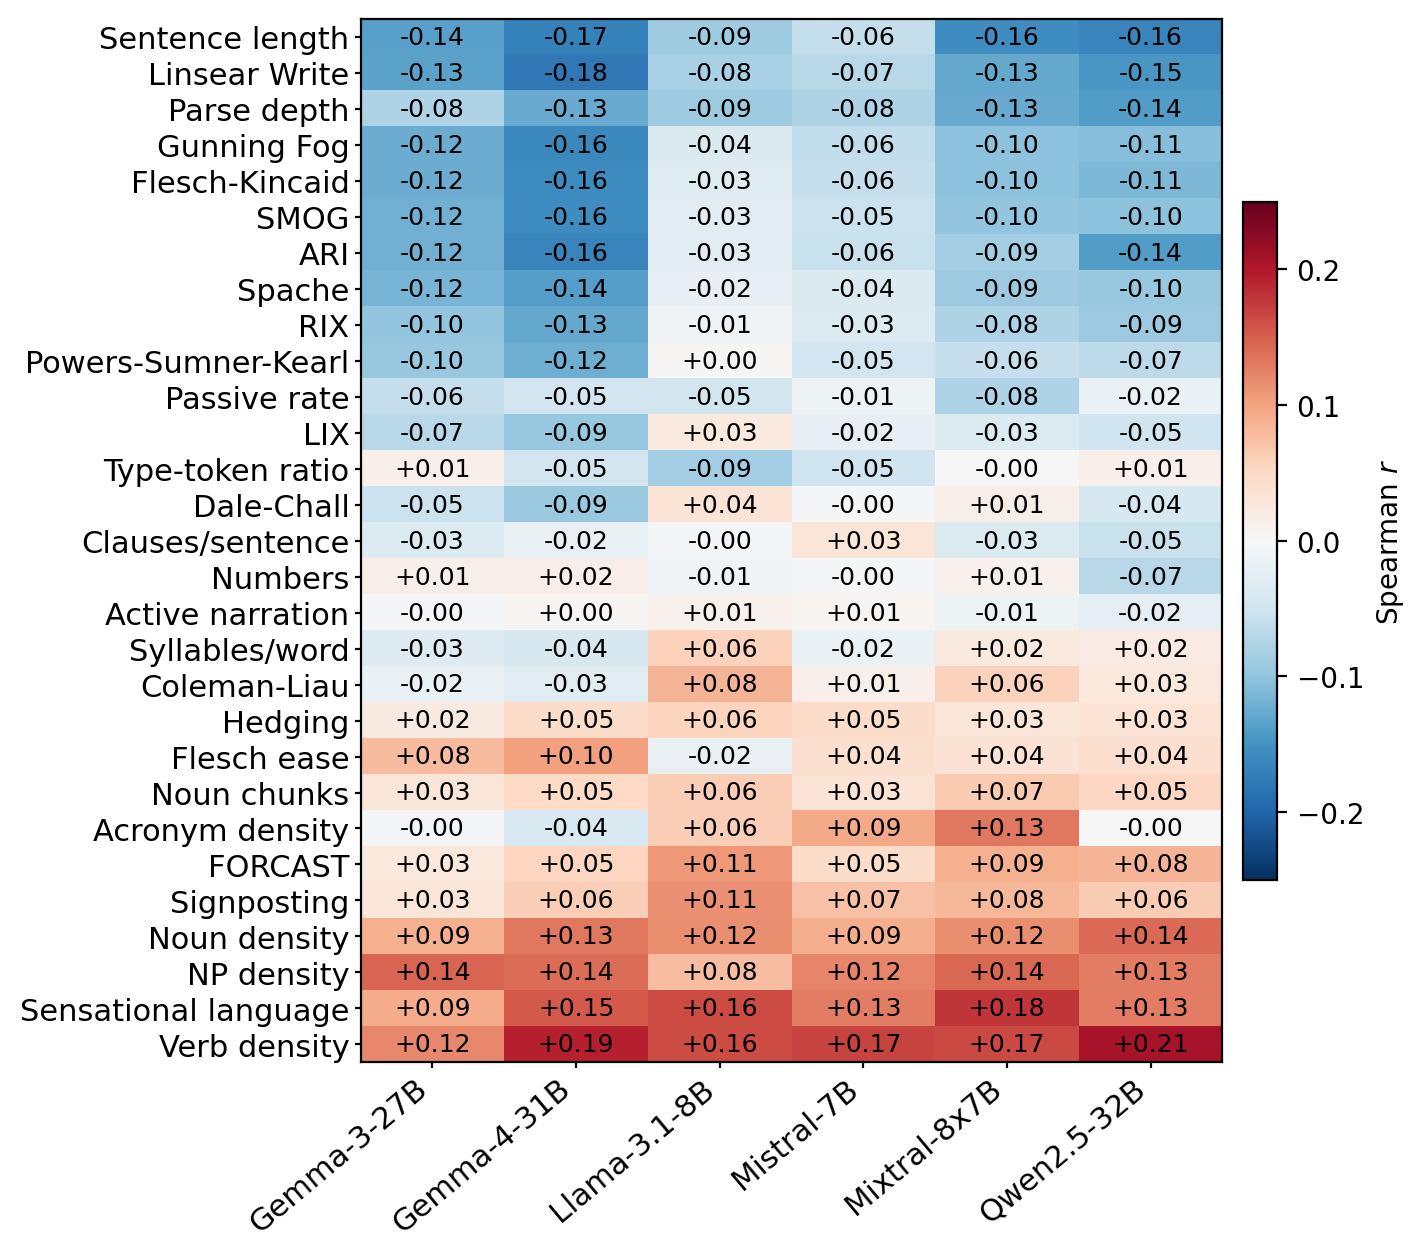
\includegraphics[width=0.82\linewidth]{../../shared/figs/fig_judge_metric_heatmap.png}
\caption{\textbf{What the LLM judge correlates with.} Per-paper Spearman
  correlation between each writing metric and each model's judge score, over
  24,754 NeurIPS abstracts. A model's score for an abstract is the median of
  its nine generations, three prompts by three sampled runs. Rows are sorted
  by the correlation with the mean of those six per-model scores
  (1987--2024, the years the judge was scored). The judge score runs 1 to 5
  with higher meaning easier, so each cell's sign says which way that feature
  moves the judge. \textbf{Red (positive): more of that feature is judged
  \emph{more} readable}, as for verb density, sensational language and noun
  phrase density. \textbf{Blue (negative): more of it is judged \emph{less}
  readable}, as for sentence length and syntactic complexity, which is the
  direction the classical formulas also take. Near-white cells, including
  acronym density, indicate near indifference. These are correlations, not
  causal claims, and every effect is small ($|r| < 0.25$).}
\label{fig:judge-tracks}
\end{figure}


\end{document}
